El servidor principal está diseñado con Spring Boot. El sistema fue implementado con una arquitectura en capas, es decir, cada capa tiene una responsabilidad específica. Las capas en las que está dividido el servidor son:
\begin{itemize}
	\item Capa de presentación: Se encarga de manejar las solicitudes HTTP, la interacción con el usuario y la presentación de los datos. Aquí entran en juego los archivos controlador, es decir, los que tienen la anotación @Controller y @RestController.
	\item Capa de negocio o servicio: Contiene la lógica de negocio central de la aplicación. Los archivos de servicio son los que se encargan de manejar todas las operaciones y las que interactúan con la capa de persistencia. Estos archivos presentan la anotación @Service.
	\item Capa de persistencia: Maneja la interacción con la base de datos. Las clases encargadas de esto son los archivos repositorio, es decir, los que tienen la anotación @Repository, o, en su defecto, las que extienden interfaces de Spring Data JPA.
	\item Capa de Base de Datos: Es decir, la capa en donde se almacenan todos los datos.
\end{itemize}
La comunicación entre cada una de estas capas se realiza mediante objetos DTO, mientras que se comunica con otros servicios mediante servicios REST. Por otra parte, es importante mencionar que para la implementar la base de datos, se hizo uso de JPA para el mapeo de las clases a las tablas dentro de la base de datos.

Se definieron entidades como `Alumno`, `UnidadAcademica` y `UnidadAprendizaje`, las cuales tienen la anotación @Entity y son mapeadas a tablas PostgreSQL. La relación entre tablas se configuró con anotaciones @OneToMany, @ManyToOne, entre otras. 

Por otro lado, para la capa de persistencia, como se mencionó anteriormente, se usaron archivos repositorio, los cuales son interfaces que extienden de JpaRepository, los cuales permiten el acceso a datos sin necesidad de usar SQL manual.

En los servicios se crearon archivos tales como AlumnoServicio, DocenteServicio, entre otros, en los cuales se encargan de guardar nuevos registros, realizar consultas o incluso actualizaciones.

Por último, los controladores, que como se mencionó, son los que se encargan de recibir peticiones HTTP y de devolver respuestas JSON al usuario.

Adicional a esto, se utilizaron servicios externos como `Cloudinary` y `Firebase`. El primero se usó para guardar las imágenes que se toman al momento del registro de los alumnos desde la simulación del SAES, mientras que el Firebase se usó para manejar los mensajes dentro de la aplicación móvil.

A continuación, en las figuras \ref{fig:UsuarioClass}, \ref{fig:InicioSesionControlador}, \ref{fig:InicioSesionServicio}, \ref{fig:InicioSesionRepositorio} se mostrará un pequeño fragmento del código de cómo se realizó esta comunicación entre las clases del servidor.

\begin{figure}[H]
	\centering
	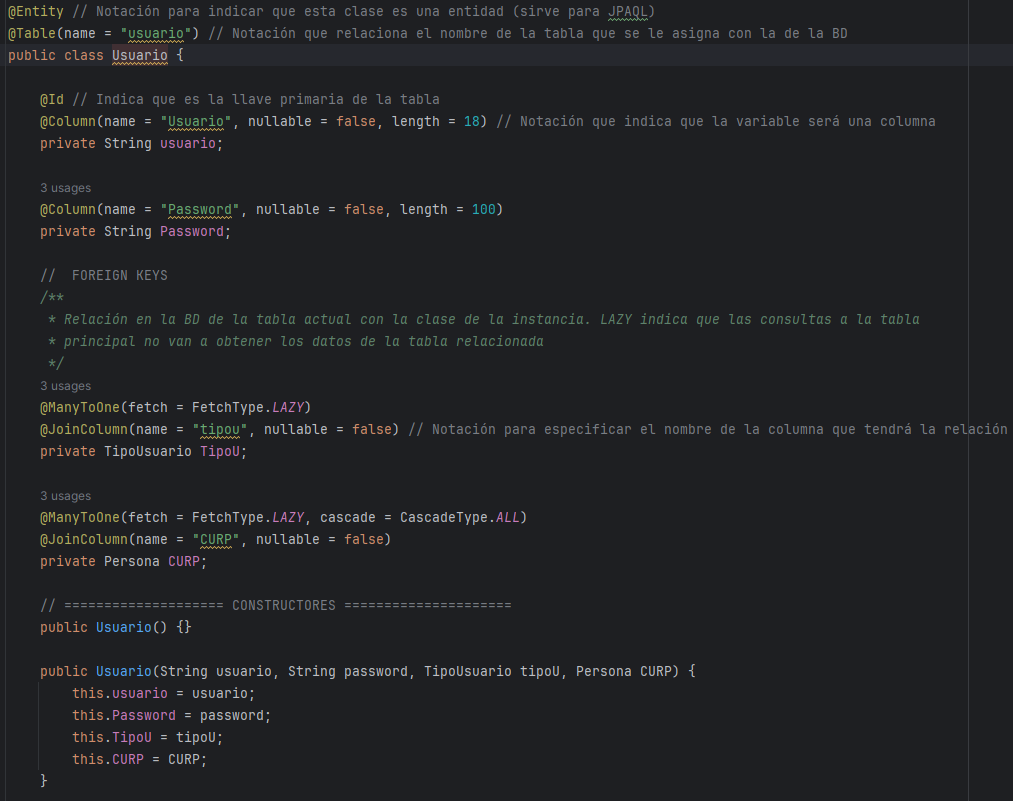
\includegraphics[width=0.7\textwidth]{images/UsuarioClass.png}
	\caption{Entidad Usuario dentro del servidor.}
	\label{fig:UsuarioClass}
\end{figure}

\begin{figure}[H]
	\centering
	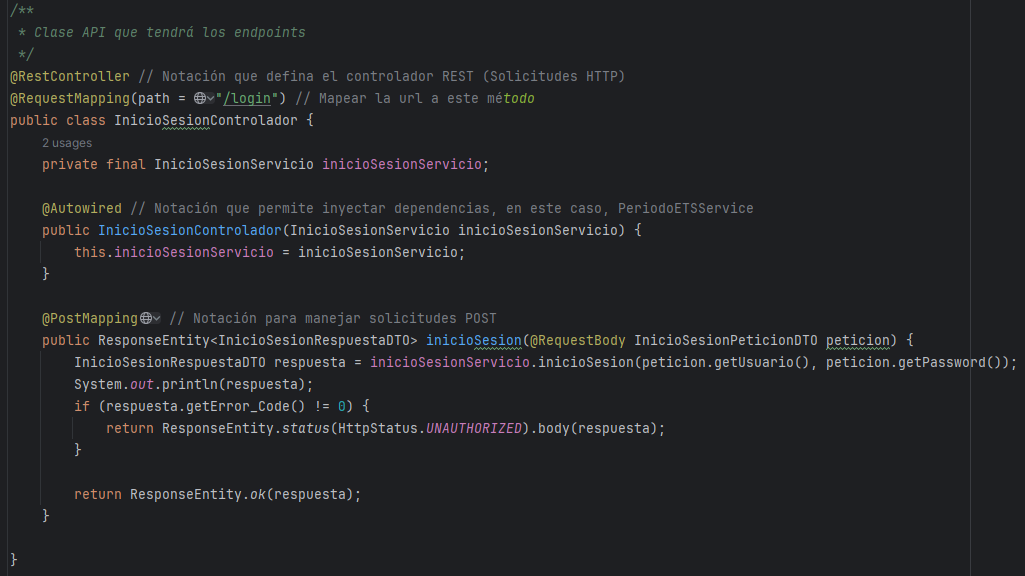
\includegraphics[width=0.7\textwidth]{images/InicioSesionControlador.png}
	\caption{Capa de presentaión (Controladores).}
	\label{fig:InicioSesionControlador}
\end{figure}

\begin{figure}[H]
	\centering
	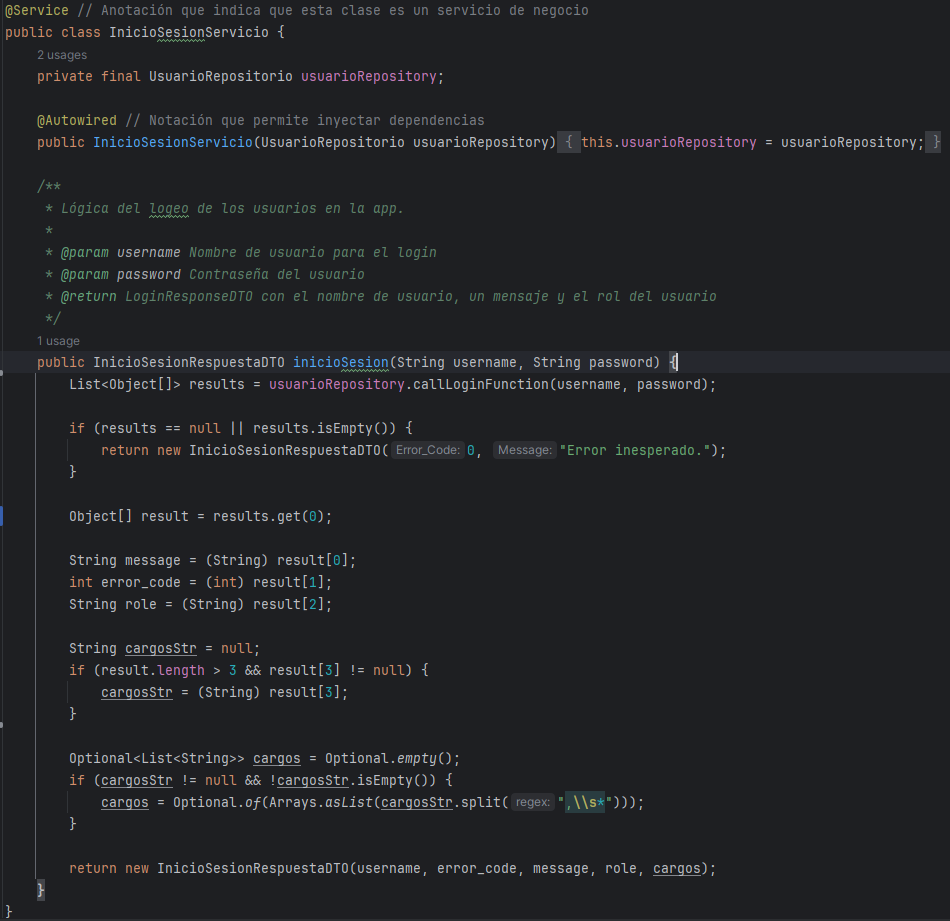
\includegraphics[width=0.7\textwidth]{images/InicioSesionServicio.png}
	\caption{Capa de negocio (Servicios).}
	\label{fig:InicioSesionServicio}
\end{figure}

\begin{figure}[H]
	\centering
	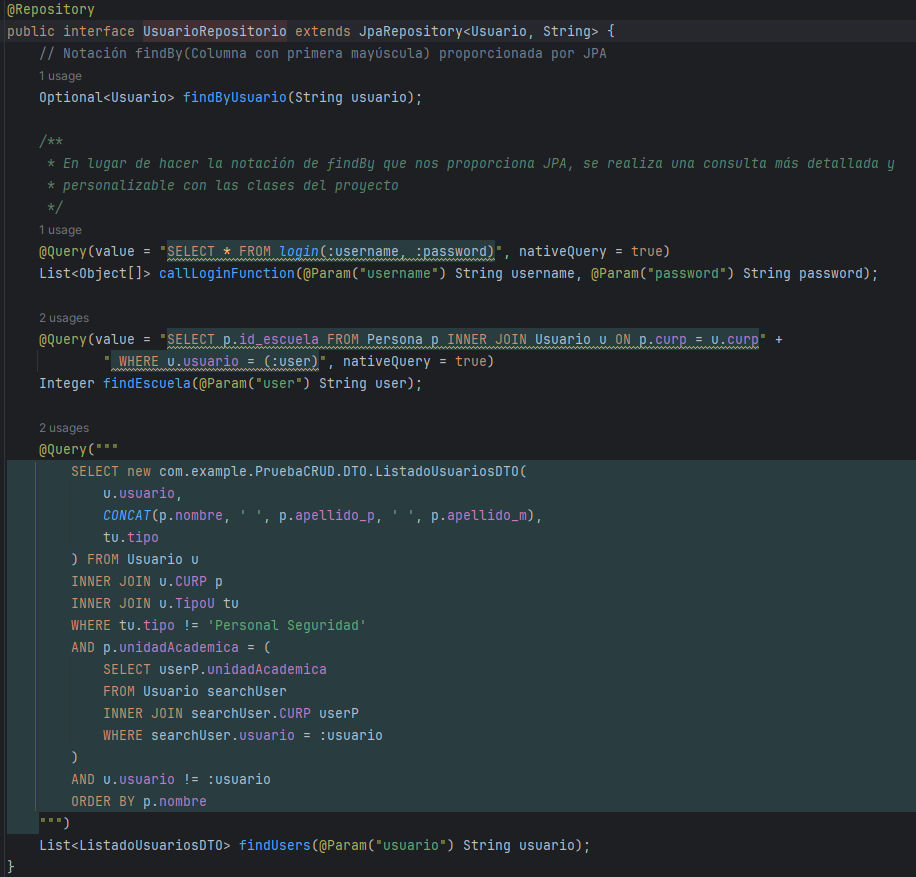
\includegraphics[width=0.7\textwidth]{images/InicioSesionRepositorio.png}
	\caption{Capa de persistencia (Repositorios).}
	\label{fig:InicioSesionRepositorio}
\end{figure}

\begin{figure}[H]
	\centering
	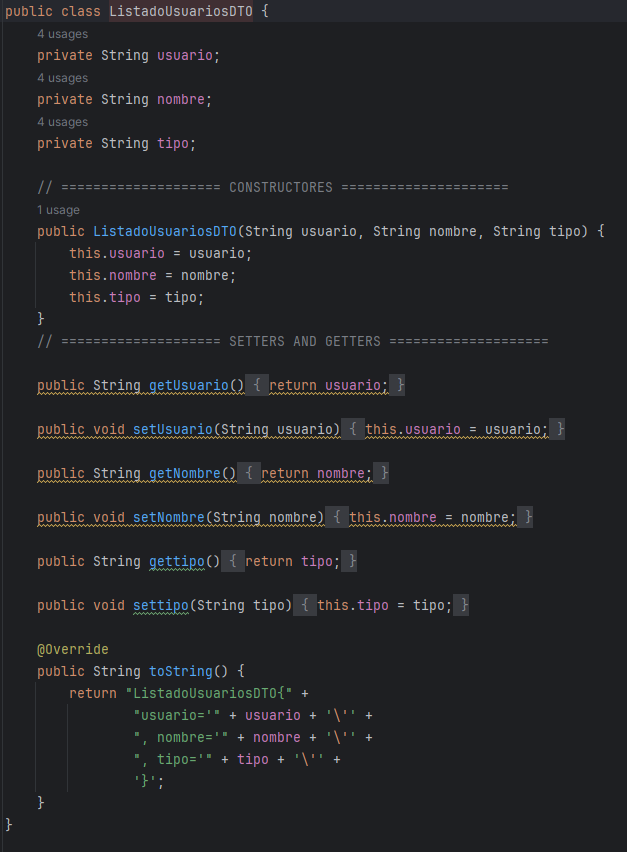
\includegraphics[width=0.7\textwidth]{images/InicioSesionDTO.png}
	\caption{Objetos DTO.}
	\label{fig:InicioSesionDTO}
\end{figure}